% vim:set spell:
% vim:spell spelllang=fr:
\documentclass[a4paper]{article}
\usepackage[utf8x]{inputenc}
\usepackage[T1]{fontenc}
\usepackage{charter}
\usepackage{helvet}
\usepackage{graphicx}
\usepackage{amsmath,amssymb}
\usepackage[french]{babel}
\usepackage{xspace}
\usepackage{setspace}
\setstretch{1.0}
\usepackage{subfigure}
\usepackage{listings}
\voffset       -1in
\hoffset       -1in
\headheight     12pt
\headsep        12pt
\topmargin      25mm
\oddsidemargin  20mm
\textwidth      170mm
\textheight     240mm
\flushbottom
\lstset{numbers=left, numberstyle=\tiny, stepnumber=1, numbersep=5pt}
\graphicspath{{../figures-1-bit/}}
\begin{document}
\begin{center}
\large
Travaux Pratiques Archi SLE-3A\\
\LARGE
Prédiction de branchements\\
\large

\end{center}
\section{Identification}
Travail réalisé par Frédéric Pétrot

\section{Prédicteur 1-bit : conception et résultats}
\subsection{code}
Le prédicteur 1 bit est constitué d'un unique tableau de booleens.
Son code est donné ci-dessous.
\small
\begin{verbatim}
// Prédicteur naïf 1-bit qui recopie la dernière décision prise
// Ajout d'une information à la class branch_update à titre d'exemple
class my_update : public branch_update {
public:
        unsigned int index;
};

class my_predictor : public branch_predictor {
   public:
      my_update u;
      branch_info bi;
      // 2^TABLE_BITS entrées de 2 bits
      // TABLE_BITS est passé sur la ligne de commande du compilateur
      unsigned char tab[1<<TABLE_BITS];

      // Constructeur
      my_predictor (void) { 
         memset (tab, 0, sizeof (tab));
      }

      // Calcul de la prédiction
      branch_update *predict (branch_info & b) {
      bi = b;
      if (b.br_flags & BR_CONDITIONAL) {
         // Saut conditionnel
         // Récupération des bits de l'adresse pour indexer la table
         u.index = (b.address & ((1<<TABLE_BITS)-1));
         // Choix de la direction (la mise à jour se fait dans update
         u.direction_prediction (tab[u.index]);
      } else {
         // Saut inconditionnel
         u.direction_prediction (true);
      }
      // Adresse prédite, si on sait le faire
      u.target_prediction (0);
      return &u;
   }

   // Mise à jour de la table de prédiction
   void update (branch_update *u, bool taken, unsigned int target) {
   // Saut conditionnel
   // On peut forcer à true ou false pour avoir les extrêmes
      if (bi.br_flags & BR_CONDITIONAL) {
         tab[((my_update*)u)->index] = taken;
      }
   }
};
// vim:se ts=3:
\end{verbatim}
\normalsize

\subsection{Résultats}
Les résultats issus de la simulation sont les suivants.
\par
\begin{minipage}{.48\linewidth}
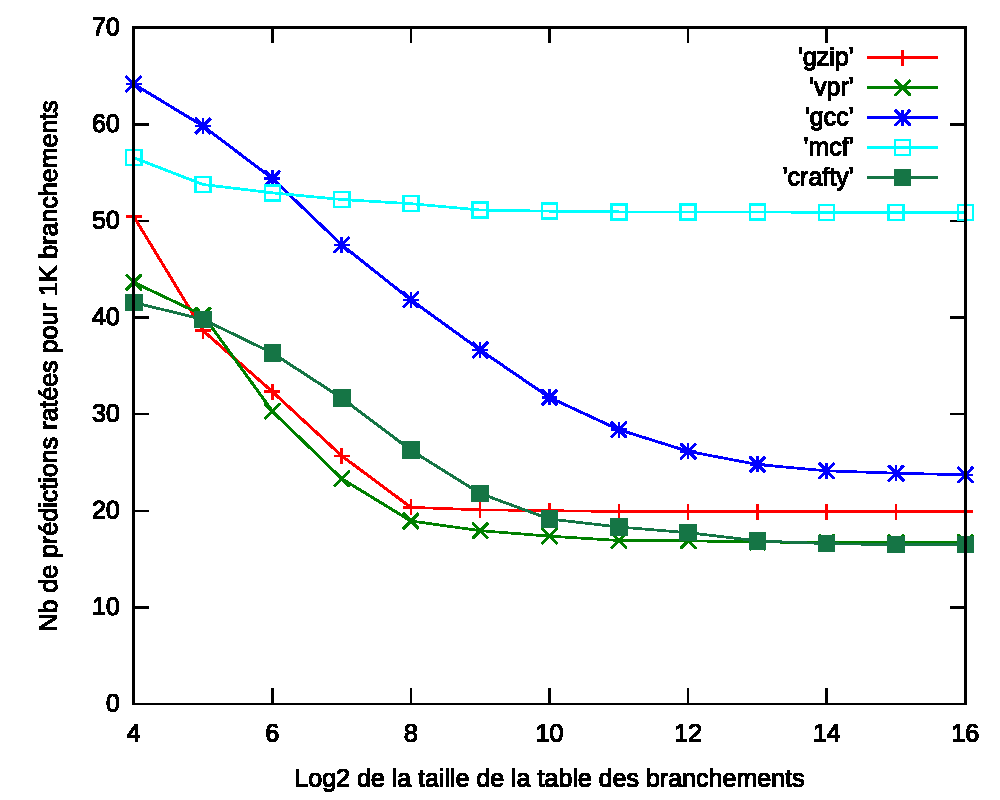
\includegraphics[width=\linewidth]{1-bit-0}
\end{minipage}%
\hfill
\begin{minipage}{.48\linewidth}
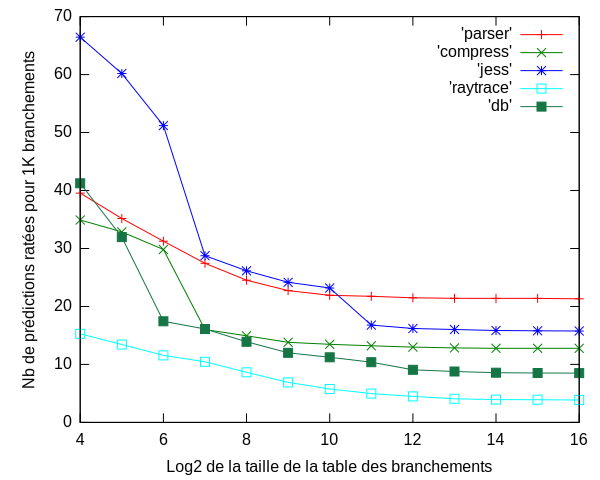
\includegraphics[width=\linewidth]{1-bit-1}
\end{minipage}

\begin{minipage}{.48\linewidth}
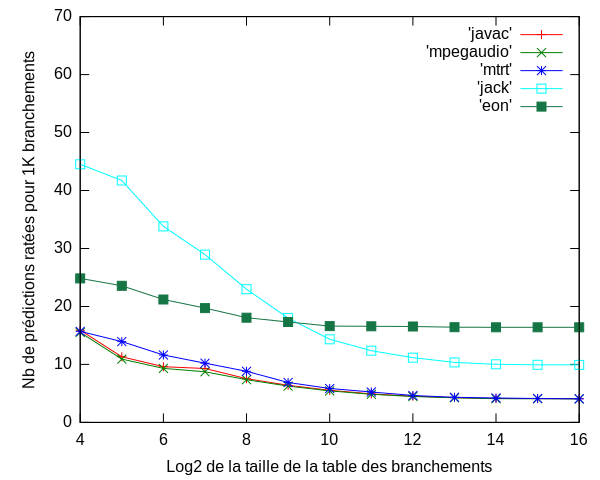
\includegraphics[width=\linewidth]{1-bit-2}
\end{minipage}%
\hfill
\begin{minipage}{.48\linewidth}
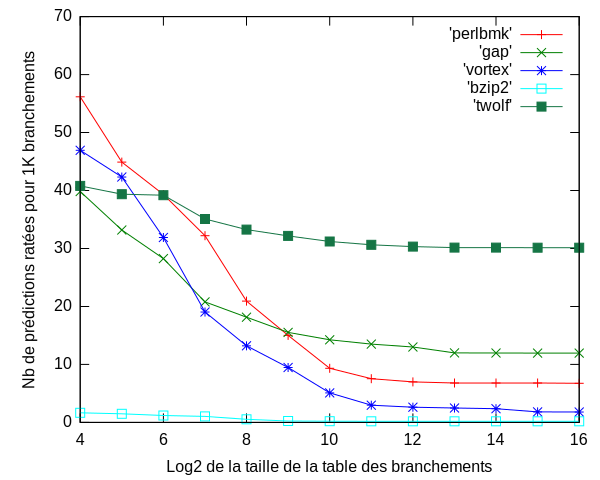
\includegraphics[width=\linewidth]{1-bit-3}
\end{minipage}
\subsection{Analyse}
On voit une asymptote due à la disparition des collisions lorsque la taille du prédicteur augmente.
Le coût du prédicteur est linéaire avec la taille du tableau, et il n'est pas raisonnable de dépasser $2^{16}$ éléments, d'autant que le gain à partir de $2^{12}$ devient très faible.
Par ailleurs, il y a toujours moins de $7\%$ de mauvaise prédictions, ce qui est remarquable pour une approche aussi simpliste.
\end{document}
